\documentclass[11pt, oneside]{article}   	% use "amsart" instead of "article" for
\usepackage{geometry}            	% See geometry.pdf to learn the layout options. 
\geometry{letterpaper, margin=1in}              	% ... or a4paper or a5paper or ... 
\usepackage{graphicx}				% Use pdf, png, jpg, or eps§ with pdflatex; use 	
\usepackage{amssymb}
\usepackage{booktabs}
\usepackage[font=small,labelfont=bf]{caption}
\usepackage{titling}
\usepackage[printwatermark]{xwatermark}
\usepackage{xcolor}
\usepackage{graphicx}
\usepackage{tikz}
\usepackage{lipsum}

\setlength{\droptitle}{-8em}

\usepackage{fancyhdr}
\pagestyle{fancy} % enable fancy page style
\fancyfoot[R]{ % right
%    \includegraphics[scale=0.9]{../ARSlogo.png}
}

\newenvironment{noindlist}
 {\begin{list}{\labelitemi}{\leftmargin=1em \itemindent=0em}}
 {\end{list}}

\rhead{\includegraphics[width=1cm]{/home/markrobertson/mrworkspace/reports/Tuolumne/figs/logo.png}}


\title{ {\color{red} DRAFT } \\ \VAR{REPORT_TITLE|e} \\
Water Year \VAR{WATERYEAR|e} \\ \VAR{START_DATE|e} to \VAR{END_DATE|e} \VAR{FORE_DATE|e}
}

\author{USDA Agricultural Research Service, Boise, Idaho\\
NRCS National Water and Climate Center, Portland, Oregon\\
\emph{in cooperation with} U.S. Bureau of Reclamation, Boise, Idaho}
\date{}							% Activate to display a given date or no date

%\newsavebox\mybox
%\savebox\mybox{\tikz[color=red,opacity=0.3]\node{DRAFT};}
%\newwatermark*[
%allpages,
%angle=45,
%scale=6,
%xpos=-20,
%ypos=15
%]{\usebox\mybox}

\begin{document}
\maketitle

\begin{tikzpicture}[remember picture,overlay]
\node[anchor=west,inner sep=0pt] at (-1.5,4cm) {\includegraphics[height=3.5cm]{/home/markrobertson/mrworkspace/code/SNOWAV/report/figs/logo.png}};
\end{tikzpicture}

\vspace{-1.2cm}
\section{Summary}
\VAR{SUMMARY|e}

\begin{table}[h!]
\centering
\begin{tabular}{l c c c c }
\toprule
\bf{Basin} 		& SWE [\VAR{UNITS|e}]	& SWE AVAIL [\VAR{UNITS|e}] & $\Delta$SWE [\VAR{UNITS|e}] & SWI [\VAR{UNITS|e}]	 \\
\midrule
Total			& \VAR{TOTAL_SWE|e} 	& \VAR{TOTAL_SWE_AV|e} & \VAR{TOTAL_SWEDEL|e} 	& \VAR{TOTAL_SWI|e} \\
Tuolumne	    		& \VAR{SUB1_SWE|e} 	& \VAR{SUB1_SWE_AV|e}  & \VAR{SUB1_SWEDEL|e} 	& \VAR{SUB1_SWI|e} \\
Cherry	    		& \VAR{SUB2_SWE|e} 	& \VAR{SUB2_SWE_AV|e}  & \VAR{SUB2_SWEDEL|e} 	& \VAR{SUB2_SWI|e} \\
Eleanor	        & \VAR{SUB3_SWE|e} 	& \VAR{SUB3_SWE_AV|e}  & \VAR{SUB3_SWEDEL|e} 	& \VAR{SUB3_SWI|e} \\
\bottomrule
\end{tabular}
% \caption{yupperdep}
\label{tab:snotel}
\end{table}

\begin{itemize}
\item[] SWE: total snow storage in the basin.
\item[] SWE AVAIL: amount of isothermal snow, which will melt with any additional energy inputs.
\item[] $\Delta$SWE: change in SWE during the reporting period.
\item[] SWI: Snow Water Input, the combination of snowmelt and rain, during the reporting period.
\end{itemize}

\clearpage

%%  \section{Current Model Results (through \VAR{END_DATE|e}, 2017)}
\section{Results}
\VAR{RESULTS_SUMMARY|e}

% SWE change
\begin{figure}[htbp]
\begin{centering}
	% \hspace*{-.7in}
	\includegraphics[width=0.92\textwidth]{\VAR{FIG_PATH}\VAR{CHANGES_FIG}}
	\caption{Change in SWE during the reporting period.}
	\label{fig:RESULTS}
\end{centering}
\end{figure}

% SWI
\begin{figure}[htbp]
\begin{centering}
	% \hspace*{-.7in}
	\includegraphics[width=0.92\textwidth]{\VAR{FIG_PATH}\VAR{SWI_FIG}}
	\caption{Current Snow Water Inputs (SWI) for the reporting period.}
	\label{fig:SWI}
\end{centering}
\end{figure}

% SWE distribution
\begin{figure}[htbp]
\begin{centering}
	% \hspace*{-.7in}
	\includegraphics[width=0.9\textwidth]{\VAR{FIG_PATH}\VAR{RESULTS_FIG}}
	\caption{Current distribution of SWE and cold content.}
	\label{fig:RESULTS}
\end{centering}
\end{figure}

% SWE elevation
\begin{figure}[htbp]
 \begin{centering}
 	% \hspace*{-.7in}
 	\includegraphics[width=0.9\textwidth]{\VAR{FIG_PATH}\VAR{ELEV_FIG}}
 	\caption{Current SWE per elevation band for each sub basin.}
 	\label{fig:RESULTS}
 \end{centering}
\end{figure}



\clearpage

% 
\begin{figure}[htbp]
	\begin{centering}
		% \hspace*{-.7in}
		\includegraphics[width=0.9\textwidth]{\VAR{FIG_PATH}\VAR{TOTALS_FIG}}
		\caption{Daily SWE and SWI basin totals.}
		\label{fig:TOTALS}
	\end{centering}
\end{figure}

\noindent\textbf{STATEMENT OF INTENT:} This report is created as a product of a research agreement between the USDA-ARS Northwest Watershed Research Center and the NRCS National Water and Climate Center. 
This report is intended to demonstrate the capabilities of real time physically-based snow modeling and the tools being developed within the scope of that research agreement.
USDA-ARS provides the data to the best of its knowledge and shall not be liable for any consequences of any kind, including, but not limited to, lost revenues and profits, that arise from using the products provided.

Contact: Mark Robertson mark.robertson@ars.usda.gov, office phone (208) 422-0739. 

\end{document}  